%%%%%%%%%%%%%%%%%%%%%%%%%%%%%%%%%%%%%%%%%%%%%%%%%%%%%%%%%%%%%%%%%
% Tese de Doutorado / Dept. Fisica, CFM, UFSC                   %
% Lacerda@CórregoGrande - Jan/2018                              %
%%%%%%%%%%%%%%%%%%%%%%%%%%%%%%%%%%%%%%%%%%%%%%%%%%%%%%%%%%%%%%%%%

%:::::::::::::::::::::::::::::::::::::::::::::::::::::::::::::::%
%                                                               %
%                          Capítulo 3                           %
%                                                               %
%:::::::::::::::::::::::::::::::::::::::::::::::::::::::::::::::%

%***************************************************************%
%                                                               %
%                          DIG class                            %
%                                                               %
%***************************************************************%

\chapter{Classificação}
\label{sec:DIGclass}
Nosso objetivo neste trabalho é desenvolver uma maneira de caracterizar as regiões de galáxias pelo seu regime de ionização, ou seja, separar regiões SF e DIG, diferenciar componentes do DIG e ir além, servir de legado para futuros trabalhos que possam utilizar essa classificação no estudo do comportamento de diferentes propriedades estelares sob distintas componentes do ISM. Com isso poderemos, através de comparações com os espectros integrados, resolver o {\em conumdrum} envolvendo a espectroscopia de uma fibra (ver Seção \ref{sec:intro:partes}). Neste capítulo apresentaremos o processo de classificação e os estudos em que nos embasamos para tal propósito.
% o víes causado pela mistura dessas diferentes componentes nas assinaturas espectrais,

\section{O papel de $W_{H\alpha}$ na classificação das regiões: hDIG, mDIG e SFc}
\label{sec:DIGclass:WHa}

Trabalhos anteriores utilizaram o brilho superficial de \Ha na intenção de separar regiões SF e DIG. Por exemplo \citet{Zhang.etal.2017a} argumenta que para os dados do MaNGA \citep{Bundy.etal.2015}, {\em spaxels} onde $\Sigma_{\Ha} > \Sigma_{\Ha}^{\rm SF,min} = 10^{39}$ erg$\,$s$^{-1}\,$kpc$^{-2}$ são confiavelmente dominados por SF.

Como dissemos anteriormente, nós preferimos classificar as regiões entre SF e DIG baseados em $W_{\Ha}$. Vemos na classificação utilizando $\Sigma_{\Ha}$ um erro conceitual que pode ser explicado com um pequeno experimento teórico.

Imagine dois elementos de volume dominados por DIG, ambos com área superficial $A$ emitindo um fluxo $F_{\Ha}=A\times\Sigma_{\Ha}$, como na Figura \ref{fig:DIGDIG}. Assuma que o meio é opticamente translúcido para os fótons de \Ha (não há extinção), como é apropriado para regiões de DIG, de maneira que o volume inteiro seja visto. Obviamente uma operação de soma com duas regiões DIG não deve alterar a natureza da região observada. Quando vemos uma região ao lado da outra, medimos o mesmo brilho superficial, pois temos duas vezes o mesmo fluxo e duas vezes a mesma área, $\Sigma_{\Ha}=(2 \times F_{\Ha})/(2 \times A)$, mantendo uma possível classificação através de um limite no brilho superficial válida. Por outro lado, quando vemos os dois elementos sobrepostos (ambos sobre a mesma linha de visada) medimos o dobro do brilho superficial, $\Sigma_{\Ha}=(2 \times F_{\Ha})/A$, fazendo com que uma operação DIG+DIG possa resultar em SF, conceitualmente errada.
%Esse viés é conceitualmente errado, pois duas regiões DIG sobrepostas deveriam continuar sendo classificadas como DIG.
Uma classificação utilizando $W_{\Ha}$ não carrega essa inconsistência por construção pois a largura equivalente final é a mesma independente da forma que os elementos são vistos.

Como veremos na Seção \ref{sec:DIGdisc:compare}, nos bojos de galáxias, onde há um percurso óptico maior, essa diferença nos critérios de classificação tem particular importância, podendo levar $\Sigma_{\Ha} > \Sigma_{\Ha}^{\rm SF,min}$ mesmo em absência de formação estelar.

De forma independente, podemos argumentar também que propriedades que possuam uma dependência radial, como cor, densidade de massa estelar, quantidade de gás, entre outras, fazem com que uma classificação usando um limite constante não seja apropriada para todas as partes de uma galáxia. Particulamente, quando o regime de ionização do DIG é orquestrado por HOLMES, a razão do número de fótons que podem ionizar \Ha por massa estelar é basicamente constante, gerando $W_{\Ha} \sim 1$ \AA\ independentemente dos fluxos envolvidos (\citealt{Binette.etal.1994a}; \citealt{CidFernandes.etal.2011a}; \citealt{Belfiore.etal.2016}; ver também a Seção \ref{sec:more:kSFR}). Dessa forma é fácil entender que, quando o parâmetro é um limite constante em $\Sigma_{\Ha}$, regiões DIG ionizadas por HOLMES (hDIG) com \Ha muito brilhante possam ser erroneamente classificadas como SF. Da mesma forma podemos ter regiões SF fracas classificadas como DIG devido a um baixo $\Sigma_{\Ha}$.

\edu{\ojo should I write an extensive-intensive note?} %Usando a termodinâmica como analogia, em ambos os argumentos anteriores, é a natureza extensiva de $\Sigma_{\Ha}$ que faz com haja a propensão para classificação errada entre DIG e SF. $W_{\Ha}$, por outro lado, se comporta como uma grandeza intensiva. Em termodinâmica, propriedades intensivas são aquelas que dependem


\section{A distribuição observada de $W_{H\alpha}$ e a componente hDIG}
\label{sec:DIGclass:WHaDistrib_hDIG}

%---------------------------- Figure ----------------------------
\begin{figure*}
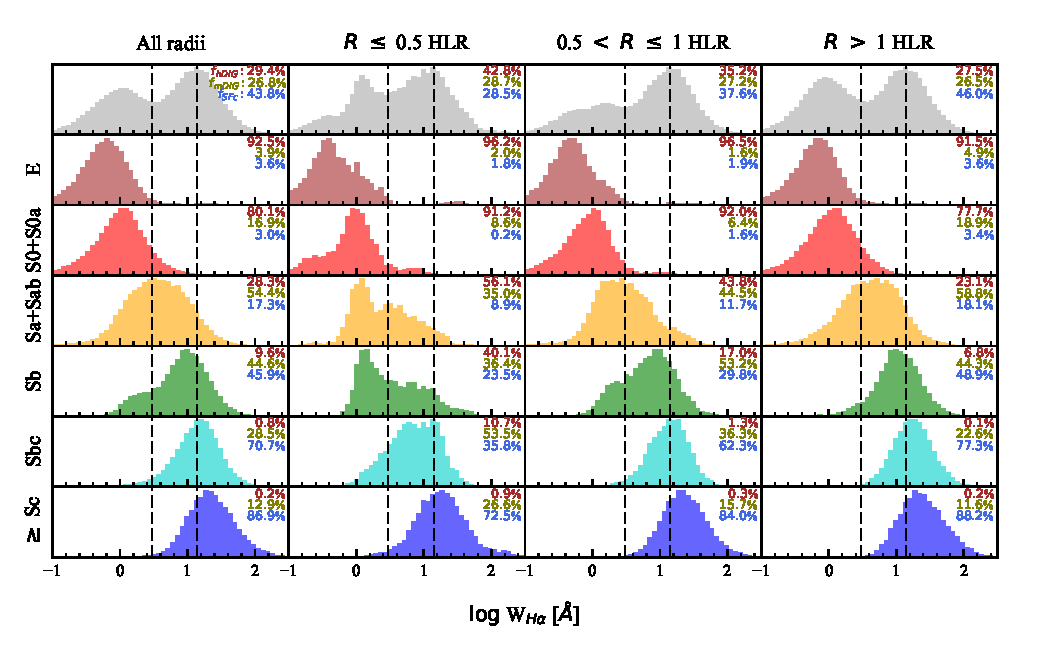
\includegraphics[scale=0.9]{figuras/fig_WHa_histograms_per_morftype_and_radius_cumulFHa.pdf}
\caption[Histogramas de $W_{H\lpha}$]
{Distribuição de $W_{\Ha}$ entre $307\,958$ zonas de 391 galáxias do CALIFA. A amostra está segmentada pela classificação de Hubble, de elípticas (segunda linha) até Sc ou mais tardias (última linha). Resultados para a amostra completa estão na primeira linha. Histogramas na primeira coluna identificam regiões de todas as partes das galáxias. Demais colunas selecionam diferentes intervalos em raio: os primeiros 0.5 HLR internos (segunda coluna), $R = 0.5$--1 HLR (terceira) e regiões exteriores com $R > 1$ HLR (quarta). Linhas tracejadas verticais marcam 3 e 14 \AA\,, as divisões entre hDIG/mDIG e mDIG/SFc respectivamente. Os números em cada gráfico representam a fração do fluxo de \Ha associada a cada componente (valor médio entre as zonas das galáxias apresentadas em cada painel).}
 \label{fig:WHaDistrib_ALLgals}
\end{figure*}
%---------------------------- Figure ----------------------------

A Figura \ref{fig:WHaDistrib_ALLgals} mostra a distribução observada de $W_{\Ha}$ para $\sim$ 300 mil zonas de 391 galáxias. Na primeira linha temos a amostra inteira e nas linhas seguintes classificamos as zonas conforme a morfologia da galáxia de onde a zona pertence; (6 classes morfológicas: E, S0-S0a, Sa-Sab, Sb, Sbc e $\ge$ Sc). Na primeira coluna temos dados de todas as regiões das galáxias, nas demais colunas classificamos as zonas por intervalos de diferentes raios: $R$ $\le$ 0.5 HLR, 0.5 < $R$ $\le$ 1 HLR, $R$ > 1 HLR.

Podemos ver que o histograma com todas as regiões de todas as galáxias (painel topo esquerdo) é claramente bimodal. Podemos distinguir duas populações com picos em $\sim 1$ \AA\ (baixo $W_{\Ha}$) e $\sim 14$ \AA\ (alto $W_{\Ha}$).
\edu{Seria interessante colocar uma figura com o ajuste gaussiano?} Esse comportamento já foi verificado utilizando dados de galáxias do \SDSS \citep{Bamford.etal.2008a, CidFernandes.etal.2011a}. Trabalhos anteriores com dados espacialmente resolvidos do CALIFA \citep{Morisset.etal.2016} e do MaNGA \citep{Belfiore.etal.2016, Belfiore.etal.2017} também identificaram essa bimodalidade.

%Antes de prosseguir, devemos dizer que estudamos também os mesmos histogramas sem a binagem espacial (todos os {\em spaxels}). Como a área é proporcional a $R^2$, o número de {\em spaxels} aumenta quando aumentamos a distância. Devido a prevalencia de regiões de formação estelar nos discos de galáxias espirais ($\ge$ Sb; $R > 1$)
%, maior número presente na nossa amostra,
%Como as regiões presentes nas regiões exteriores de galáxias espirais ($\ge$ Sa), maior número presente na nossa amostra, são dominadas por SF,
%ocorre um aumento na amplitude relativa entre os picos das duas populações, porém a bimodalidade se mantém. Vemos que há um aumento de quase três vezes dessa população, enquando, na população de baixo $W_{\Ha}$, o aumento é de apenas $\sim 20\%$. Como anteriormente, o histograma de todos os dados pode ser ajustado utilizando duas gaussianas, identificando duas componentes com centros em $\sim 1$ e $14$ \AA.

Antes de prosseguir, devemos dizer que estudamos também os mesmos histogramas utilizando os dados sem binagem espacial (todos os {\em spaxels}). Identificamos um aumento na amplitude relativa entre os picos das duas populações, porém a bimodalidade se mantém. Isso ocorre pois a área de uma galáxia é proporcional a $R^2$, assim o número de {\em spaxels} cresce quadráticamente quando aumentamos a distância ao centro. Como vemos na Figura \ref{fig:WHaDistrib_ALLgals}, devido a prevalência de regiões de formação estelar nos discos de galáxias espirais, esse aumento na amplitude relativa é um fenômeno esperado. Observamos um aumento de quase três vezes no número de regiões de alto $W_{\Ha}$ com $R > 1$ HLR nas galáxias Sb e mais tardias, enquanto, na população de baixo $W_{\Ha}$, o aumento é de apenas $\sim 20\%$. Como anteriormente, o histograma de todos os dados pode ser ajustado utilizando duas gaussianas, identificando duas componentes com centros em $\sim 1$ e $14$ \AA.

%, maior número presente na nossa amostra,
%Como as regiões presentes nas regiões exteriores de galáxias espirais ($\ge$ Sa), maior número presente na nossa amostra, são dominadas por SF,
%ocorre

Nossa interpretação é que essa população com baixas larguras equivalentes é formada por regiões DIG fotoionizadas por HOLMES. Como teste, podemos calcular $\xi$, a razão entre a luminosidade de \Ha observada e aquela esperada pelos fótons produzidos pelas populações mais velhas que $10^8$ anos, através da análise com o \starlight, seguindo a metodologia aplicada em \citet{CidFernandes.etal.2011a}. Como os modelos de populações estelares utilizados pela síntese \citep{Gonzalezdelgado2005, Vazdekis2010} não possuem a parte ionizante nos espectros ($h\nu \ge 13.6$ eV) tomamos emprestado aqueles de \citet{Bruzual.Charlot.2003} utilizando uma função inicial de massa ({\em initial mass function}; IMF) de Salpeter e as trilhas estelares de \citet{Girardi2000}. Como discutido em \citet{CidFernandes.etal.2011a} distintos modelos produzem diferenças sistematicas de 0.2--0.5 dex na quantidade  prevista de fótons ionizantes. A Figura \ref{fig:WHa-Xi} mostra $\xi$ em função de $W_{\Ha}$, com os histogramas coloridos por nossa classificação hDIG/mDIG/SFc. Verificamos que $\xi$ é de ordem 1 para as regiões com baixo $W_{\Ha}$. Consequentemente, apesar de todas as incertezas envolvidas nesse cálculo \citep{CidFernandes.etal.2011a, Belfiore.etal.2016, Morisset.etal.2016}, o resultado final corrobora a interpretação de que HOLMES são responsáveis pela população de baixo $W_{\Ha}$.

% Seja $L_{\Ha}$ a luminosidade observada de \Ha e $L_{\Ha}^{\rm exp}(t > 10^8 {\rm anos})$ a luminosidade esperada pelas populações velhas, definimos a razão como:
% \begin{equation}
%   \xi\ =\ \frac{L_{\Ha}}{L_{\Ha}^{\rm exp}(t > 10^8 {\rm anos})}.
% \end{equation}
% \noindent Podemos definir

%---------------------------- Figure ----------------------------
\begin{figure}
 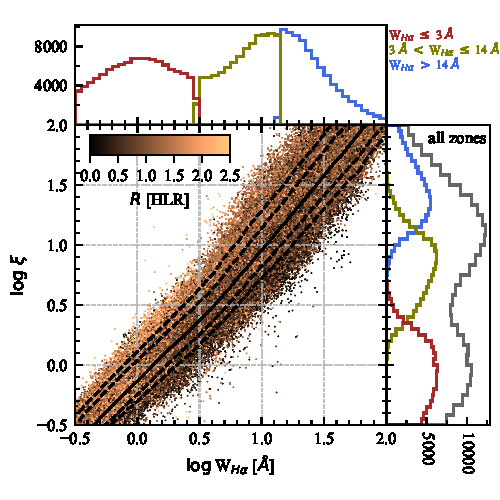
\includegraphics[scale=1.5]{figuras/fig_logxi_logWHa_histograms.pdf}
 \caption[$\xi \times \log H_\alpha$]
 {Razão entre a luminosidade de \Ha observada e aquela predita pelas poulações mais velhas que $10^8$ anos ($\xi$) em função de $W_{\Ha}$ para todas as zonas de nossa amostra. Os pontos estão coloridos conforme a distânciada até o núcleo (em unidades de HLR). Os histogramas de $\xi$ e de $W_{\Ha}$ estão coloridos como vermelho/amarelo/azul (hDIG/mDIG/SFc), mostrando que as regiões com baixo $W_{\Ha}$ são compatíveis com ionização por HOLMES.}
 \label{fig:WHa-Xi}
\end{figure}
%---------------------------- Figure ----------------------------

Fica evidente a correspondência dessa interpretação com o conceito de galáxias aposentadas apresentado por \citet{Stasinska.etal.2008a}. Estes são sistemas que pararam de formar estrelas há muito tempo, nos quais os fótons ionizantes presentes são provenientes das estrelas que já evoluíram após o ramo assintótico das gigantes ({\em post-asymptotic giant branch; post-AGB}) e de anãs brancas, levando os valores de $W_{\Ha}$ a $\sim 1$ \AA. O limite de 3 \AA\ que cinge essa população coincide com o valor utilizado por \citet{CidFernandes.etal.2011a} para distinguir galáxias aposentadas daquelas com regime de ionização dominado por SF ou por AGN. Por esse motivo nós firmemente indicamos que as populações com $W_{\Ha} < 3$ \AA\ sejam classificadas como gás difuso ionizado por HOLMES, o hDIG.

A separação da distribuição de $W_{\Ha}$ por tipos de Hubble mostra que a bimodalidade está sempre presente, mudando apenas a proporção entre as populações de baixo e alto $W_{\Ha}$ conforme a morfologia: galáxias {\em early-type} são esmagadoramente dominadas por valores ao redor do pico de $\sim 1$ \AA, enquanto nas galáxias espirais tardias é a população com alto $W_{\Ha}$ que domina.

Quando dividimos a amostra em intervalos de $R$ vemos que a população hDIG se distribui igualmente entre as galáxias {\em early-type}, confirmando estudos anteriores de \citet{Kehrig.etal.2012}, \citet{Singh.etal.2013}, e \citet{Gomes.etal.2016b}, além das análises baseadas em dados do MaNGA por \citet{Belfiore.etal.2016, Belfiore.etal.2017}. Entre as Sb e espirais mais tardias o hDIG fica concentrado nas regiões centrais das galáxias. Para colocar isso em números, 82\% dos pontos hDIG das 225 galáxias Sb ou mais tardias estão localizados em regiões onde $R < 1$ HLR.

Nós interpretamos essa alta incidência de zonas hDIG nas regiões centrais como um corolário da prevalência de populações velhas nos bojos. Além de HOLMES, qualquer outro tipo de fonte de ionização relevante elevaria os valores de $W_{\Ha}$. Por outro lado, a baixa incidência de regiões com $W_{\Ha} < 3$ \AA\ situadas a grandes distâncias do centro ($R$ grande) em galáxias espirais indica que a emissão hDIG não é estatisticamente relevante para o DIG que permeia as regiões SF presentes em seus discos. A Figura \ref{fig:WHaDistrib_ALLgals} também mostra que apesar do hDIG explicar uma parte substancial da emissão nos discos de galáxias Sa--Sab, entre as Sb ou mais tardias são raras as incidências de discos dominados pelo hDIG.

Podemos ver que a introdução da categoria hDIG em nossa classificação é eregida sob um cenário criado por argumentos teóricos e experimentais. Essa componente do DIG está muito bem compreendida e se torna dominante sempre que HOLMES é a fonte de ionização mais relevante.

Finalizamos esta seção analisando a extensão que efeitos de inclinação podem causar na distribuição de $W_{\Ha}$. \edu{\ojo Figura?} Para esse experimento primeiro eliminamos galáxias elípticas (E e S0) de nossa amostra. Então dividimos a amostra por classes de diferentes $b/a$ (elipticidade\footnote{a razão entre o eixo maior e o eixo menor de uma elipse}, conforme cálculo detalhado em \citealt{deAmorim.etal.2017}). O único efeito digno de nota é que ao observarmos zonas com $R < 0.5$ HLR existe um efeito de projeção. Ao irmos de galáxias {\em edge-on} para {\em face-on}, os histogramas tendem a se deslocarem $\sim$ 0.2--0.3 na direção de valores mais baixos de $W_{\Ha}$. Isso acontece pois enquanto regiões centrais em galáxias {\em face-on} amostram o bojo, que tem características hDIG, ao aumentarmos a inclinação partes do disco ficam projetadas sob a linha de visada, resultando numa mistura de regiões SFc e hDIG. Porém, assim como os efeitos da binagem espacial usando zonas de Voronoi, os efeitos de inclinação também não apagam a dicotomia fundamental entre esses dois regimes nebulares.

\subsection{Identificação das componentes hDIG, mDIG e SFc}
\label{sec:DIGclass:identclass}

As populações de baixo $W_{\Ha}$ podem ser seguramente classificadas como hDIG. Diferentemente, as populações de alto $W_{\Ha}$ não podem serem identificadas univocamente como SFc. Certamente as regiões SF estão entre essas com $W_{\Ha}$ alto, porém outros processos de ionização podem guiar a disponibilidade de fótons ionizants dessas regiões. Particularmente, a ionização do DIG por fótons que escapam de regiões \hii está entre esses processos. Nesse caso, a razão de fótons ionizandes por unidade de massa estelar eleva os valores de $W_{\Ha}$ acima daqueles típicos em regiões ionizadas por HOLMES.

Sabendo que a população com alto $W_{\Ha}$ representa uma mistura de regimes, é útil subdividi-la entre mDIG e SFc, de maneira a identificar zonas onde a formação estelar é a fonte de ionização relativamente mais importante. Não existe fronteira conspícua que possa diferenciar regiões SFc de mDIG em função de $W_{\Ha}$. Como podemos ver na Figura \ref{fig:WHaDistrib_ALLgals}, a população com alto $W_{\Ha}$ é unimodal, não sugerindo a existência de subpopulações e sim de uma distribuição contínua. Na falta de um valor que possa ser usado como critério para a divisão entre mDIG e SFc utilizamos 14 \AA\ para tal classificação, coincidindo com o pico da distribuição dessa população.

Nosso esquema final de classificação é, portanto

\begin{itemize}
 \item hDIG: $W_{\Ha} \le 3 \,\mathrm{\AA}$,
 \item mDIG:  $3 \,\mathrm{\AA}  < W_{\Ha} \le 14 \,\mathrm{\AA}$,
 \item SFc: $W_{\Ha} > 14 \,\mathrm{\AA}$.
\end{itemize}

Devemos levar em conta uma assimetria conceitual nessa classificação. Enquanto a fronteira hDIG/mDIG em 3 \AA\ é firmemente ancorada em um conhecimento teórico da natureza da população hDIG, totalmente corroborada pela bimodalidade na distribuição de $W_{\Ha}$, nada nesse nível pode ser afirmado sobre a divisão entre mDIG/SFc. Tudo o que podemos dizer é que regiões com $W_{\Ha}$ acima de 14 \AA\ possuem uma maior proporção de SFc do que aquelas abaixo. Portanto, através dessa classificação, devemos considerar que as regiões mDIG podem carregar alguma formação estelar e que regiões SFc não isolam regiões SF puras. Regiões \hii gigantes genuínas, objetos base para qualquer estudo de linhas de emissão em galáxias, possuem $W_{\Ha}$ uma ordem de grandeza maior \citep{McCall.etal.1985, Garnett.and.Shields.1987, Kennicutt.and.Garnett.1996, Luridiana.and.Peimbert.2001, Bresolin.etal.2004}, porém, como mencionado anteriormente, com a resolução de nossos dados esses objetos estão muito diluídos.

Com nossas regiões classificadas podemos retornar ao painel mais à esquerda da Figura \ref{fig:ExampleMaps}. Nele vemos os mapas de $W_{\Ha}$ saturados pelos intervalos $< 3$ \AA\ (hDIG, vermelho) e $> 14$ \AA\ (SFc, azul). Cores intermediárias representam o intervalo de 3--14 \AA\ (mDIG). A galáxia S0 no topo da figura exemplifica o domínio do hDIG sobre as galáxias {\em early-type} como foi previamente inferido dos histogramas de $W_{\Ha}$ na Figura \ref{fig:WHaDistrib_ALLgals}. Através dos mapas da CALIFA 0886 (NGC 7311) e da 0010 (NGC 0036) observamos o domínio da componente hDIG nos bojos de galáxias. Como era esperado, a componente SFc se torna cada vez mais importante a medida que avançamos para tipos mais tardios na classificação de Hubble (seguindo de cima para baixo nas Figuras \ref{fig:ExampleMaps} e \ref{fig:WHaDistrib_ALLgals}).

Finalizamos este capítulo referenciando aqui o trabalho de \citet{Sanchez.etal.2015MUSE}, um exemplo de estudo embasado em imagens com uma resolução espacial muito maior, obtidas com o MUSE. Podemos ver que o mapa de $W_{\Ha}$ da galáxia NGC 6754, reproduzido aqui na Figura \ref{fig:WHaSebasMUSE}, mostra um domínio completo de regiões SFc permeadas por emissão mDIG em todo disco.

\begin{figure}
 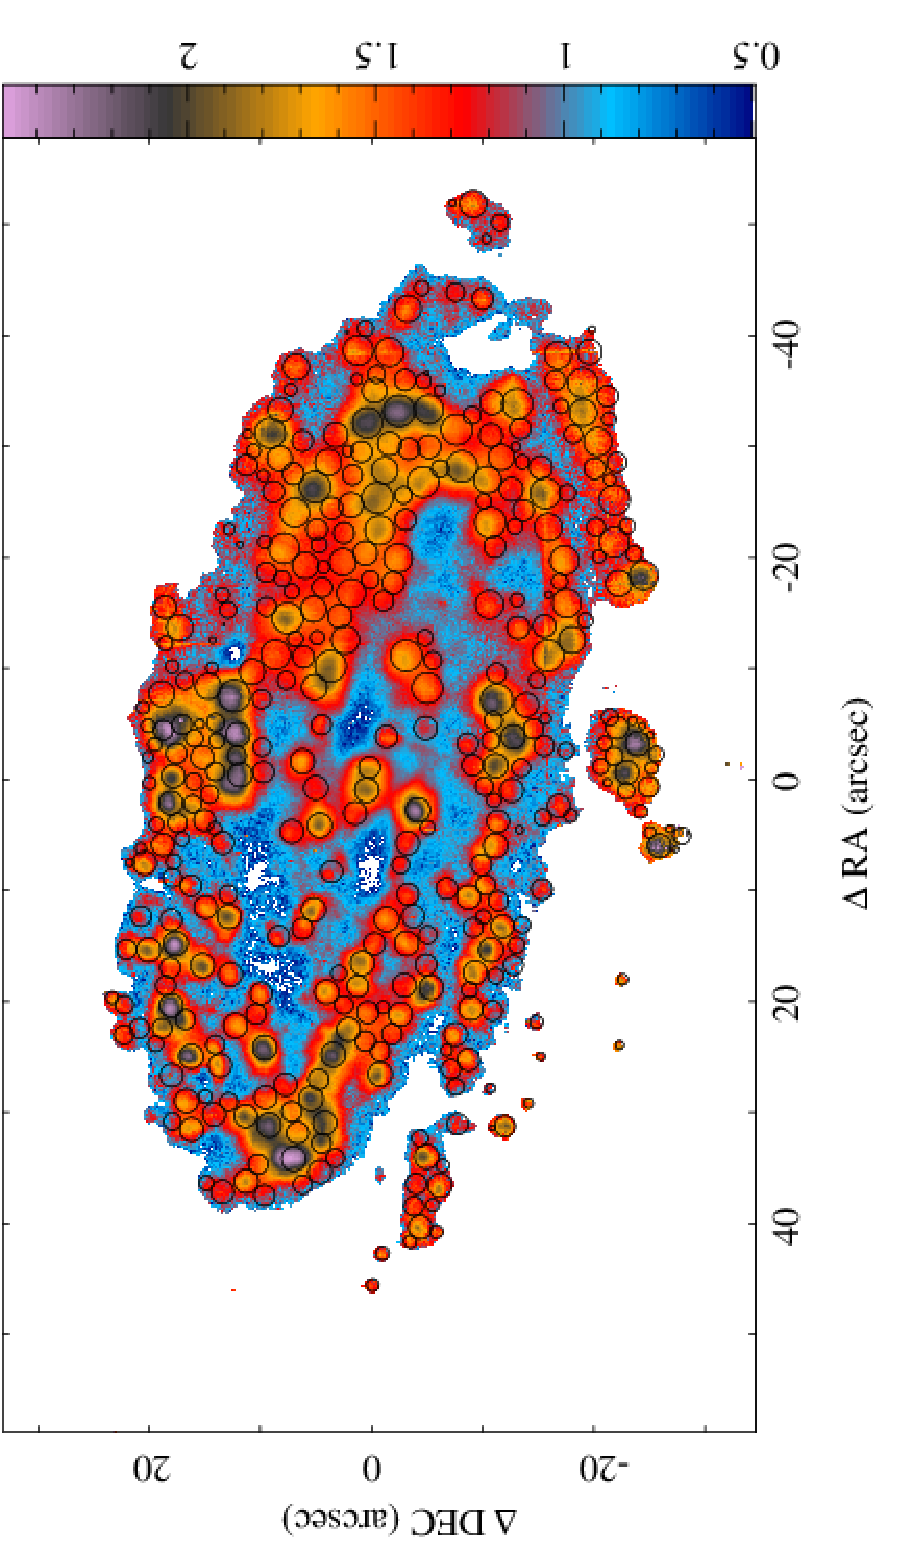
\includegraphics[scale=0.45,angle=-90]{figuras/map_EW_Ha_HII.pdf}
 \caption[MUSE: Mapa de $W_{H\alpha}$ da galáxia NGC 6754]
 {Mapa da galáxias NGC 6754 obtido por \citet{Sanchez.etal.2015MUSE} colorido por $\log\ W_{\Ha}$. Regiões com detecção de fluxo de \Ha abaixo de $\sim 3\sigma$ são mascaradas. Os circulos marcam regiões \hii detectadas.}
 \label{fig:WHaSebasMUSE}
\end{figure}


%% End of this chapter
